\documentclass[11pt, twocolumn, a4paper]{article}

\usepackage{graphicx}

\setlength{\oddsidemargin}{0.0 cm}
\setlength{\evensidemargin}{0.0 cm}
\setlength{\topmargin}{-1cm}
\setlength{\textheight}{24 cm}
\setlength{\textwidth}{16 cm}

\newcommand{\ttbar}{$\mathrm{t \overline{t} \; }$}

\pagestyle{plain}

\setlength{\parindent}{0in}

\usepackage[
  locale=DE,
  separate-uncertainty=true,
  decimalsymbol=.,
  per-mode=symbol-or-fraction,
]{siunitx}

\begin{document}

\author{Salvatore La Cagnina}

\title{Summary of `CMS Collaboration, {\it Measurements of the $\mathrm{t\overline{t}}$ production cross section using events in the $\mathrm{e\mu}$ final state in pp collisions at $\sqrt{s} = \SI{13}{TeV}$}'}

\maketitle

The paper describes the analysis of \ttbar events with $\mathrm{e\mu}$ final state in order to measure the \ttbar production cross section.
It uses data provided by the CMS experiment from pp collisions at a center of mass energy of $\SI{13}{TeV}$ with an integrated luminosity of $\SI{2.2}{fb^{-1}}$.
The selection of this analysis consists of having an opposite signed (OS) pair of electron and muon together with two or more jets of which at least one resulted from the decay of a b quark.
The measured cross section for the \ttbar production is ${\SI[parse-numbers=false]{815 \pm 9 (stat) \pm 38 (syst) \pm 19 (lumi)}{\pico\barn}}$ which is in agreement with the standard model prediction.


\section{Introduction}
Measuring the \ttbar production at the CMS experiment at the LHC yields multiple beneficial information.
It tests the prediction provided by the QCD and can add constrains on the parton distribution functions. 
Additionally, it grants information about the top quark pole mass but most important reason precise data about the \ttbar production is necessary is the search for BSM physics since \ttbar is the dominant background in those analysis.
For the analysis the full data set of 2015 from the CMS experiment is used providing a data set corresponding to an inverse luminosity of $\SI{2.2}{fb^{-1}}$.

\section{The CMS detector and Monte Carlo simulation}
The silicon pixel detector of the CMS detector covers $0 < \Phi < 2 \pi$ azimuth and a pseudorapidity of $| \eta | < 2.5$.
In order to detect jets and electron the lead tungstate crystal electromagnetic and the brass and scintillator hadron calorimeter.
Muons can be detected using the gas-ionization detectors outside the solenoid.
In order to simulate signal and background events different Monte Carlo (MC) event generators are used such as \texttt{POWHEG},\texttt{PYTHIA},\texttt{HERWIG++} and \texttt{MG5\_aMC}.
The Standard Model prediction is calculated with \texttt{TOP++} 
The main background processes for the 


\begin{thebibliography}{99}
\bibitem{paper} CMS Collaboration, Measurement of the $\mathrm{t\overline{t}}$ production cross section using events in the e$\mathrm{\mu}$ final state in pp collisions at ${\sqrt{s} = \SI{13}{TeV}}$, Eur. Phys. J. C 77 (2017) 172.
\end{thebibliography}



\end{document}


%\begin{figure}[ht!]
%  \begin{center}
%    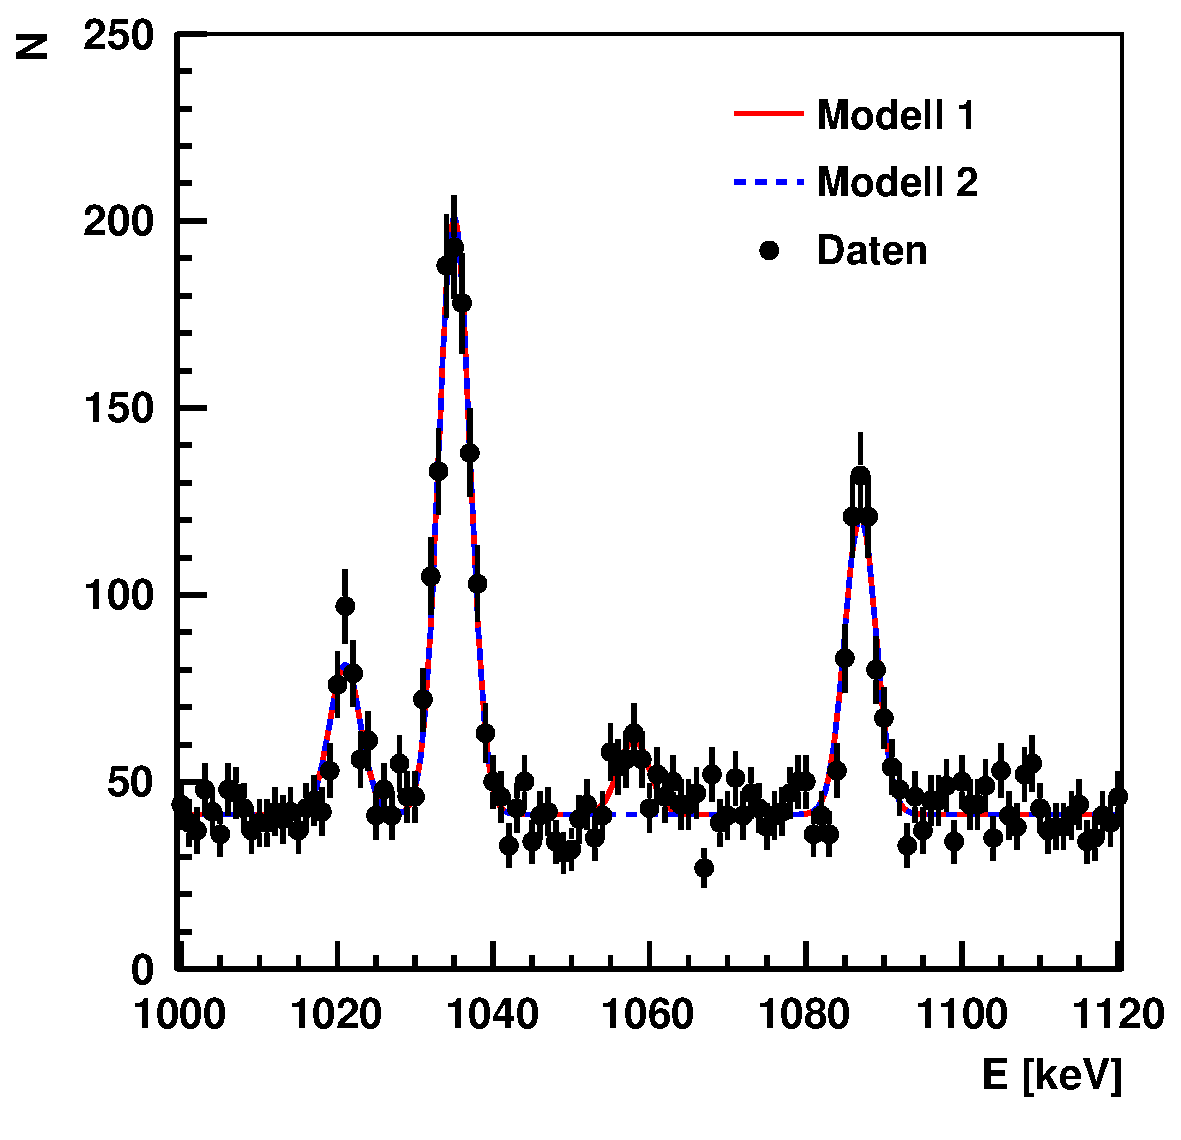
\includegraphics[width=0.5\textwidth]{plot.pdf}
%    \caption{A figure caption~\cite{brandt}.}
%    \label{fig:fig1}
%  \end{center}
%\end{figure}
